\documentclass{article} 

\usepackage{fancyhdr}
\usepackage[english]{babel}

\usepackage{fullpage}
\usepackage[margin = .75 in]{geometry}
\usepackage[leqno]{amsmath}
\usepackage{amsmath}
\usepackage{amsfonts}
\usepackage{amssymb}
\usepackage{amsthm}
\usepackage{amssymb}
\usepackage[all]{xy}
\usepackage{graphicx}

\usepackage{graphicx,color,url,hyperref}
\usepackage{epsfig}
\fancyhf{}
\setlength{\parindent}{0pt}
\setlength{\parskip}{5pt plus 1pt}
\setlength{\headheight}{13.6pt}

\newcommand{\NN}{\mathbf N}
\newcommand{\RR}{\mathbf R}
\newcommand{\CC}{\mathbf C}
\newcommand{\ZZ}{\mathbf Z}
\newcommand{\ZZn}[1]{\ZZ/{#1}\ZZ}
\newcommand{\QQ}{\mathbf Q}
\newcommand{\nn}{\mathbb N}
\newcommand{\rr}{\mathbb R}
\newcommand{\cc}{\mathbb C}
\newcommand{\zz}{\mathbb Z}
\newcommand{\zzn}[1]{\zz/{#1}\zz}
\newcommand{\qq}{\mathbb Q}
\newcommand{\calM}{\mathcal M}
\newcommand{\latex}{\LaTeX}
\newcommand{\tex}{\TeX}
\newcommand{\dd}{{\rm d}}
\newcommand{\sm}{\setminus} 

\title{Final Project}
\author{Sunny Lee and Connor Stevens}
\date{March 30, 2021}

\pagestyle{fancy}
\fancyhf{}
\rhead{March 30, 2021}
\lhead{Sunny Lee and Connor Stevens}
\chead{Final Project}
\rfoot{Page \thepage}

\begin{document}

\begin{enumerate}
    \item Using the Vandermonde matrix constructed from the $x$ vector, we can make an 
    augmented matrix with the $y$ vector given. This augmneted matrix can then be solved
    through Gaussian Elimination, and we obtain the coefficients of the degree $9$ 
    function: \\
    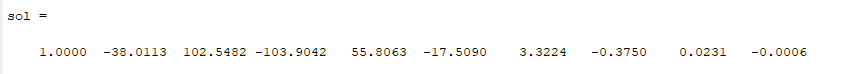
\includegraphics[scale = .7]{coefficients.png}\\
    and thus, our Lagrange polynomial is: 
    \[
        x^9-38.0113x^8+102.5482x^7-103.9042x^6+55.8063x^5-17.5090x^4+3.3224x^3-0.3750x^2+0.0231x-0.0006
    \]

    When we graph the polynomial against our data, we can see there are definitely
    some overfitting problems happening: \\
    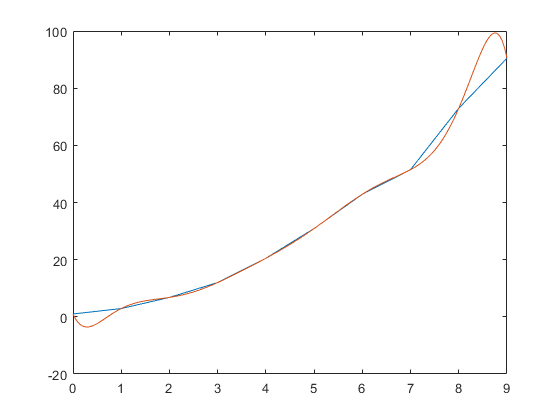
\includegraphics{number1graph.png}\\

    \item 
    \begin{enumerate}
        \item Using the normal equation where we take the inverse of $A$, we obtain
        the coefficients: \\
        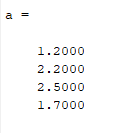
\includegraphics{number2a.png}\\
        and thus our multiple linear regression model is 
        $1.2x_1+2.2x_2+2.5x_3+1.7x_4$
        \pagebreak

        \item Using the Cholesky factorization before solving for $x$, we obtain the 
        lower triangular matrix: \\
        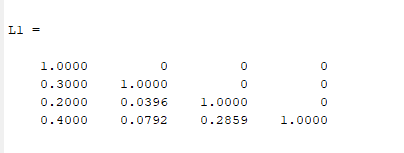
\includegraphics{2ba.png}\\
        Solving using the lower triangular matrix, we see we obtain the same result: \\
        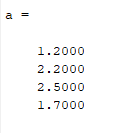
\includegraphics{number2a.png} 
    \end{enumerate}

    \item 
    \begin{enumerate}
        \item Using the Vandermonde matrix to solve for the polynomial: \\
        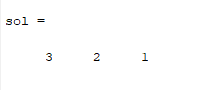
\includegraphics{3a.png}\\
        And thus, using the Vandermonde matrix, we obtain the polynomial $3x^2+2x+1$

        \item Using gradient descent, we first set our coefficients as $3.1x^2+1.9x+1.1$. 
        To estimate the coefficients we found in Part A, we must first find the gradient 
        of the cost function. For our cost function, we will be using the mean squared
        error or MSE:
        \begin{gather*}
            MSE = \frac{1}{n}\sum_{i = 1}^n{(\hat{y_i} - y_i)^2}
        \end{gather*}
        In our case, since $\hat{y} = ax^2 + bx + c$ and we are using 3 data points:
        \begin{gather*}
            \frac{1}{3}\sum_{i = 1}^3{(ax_i^2 + bx_i + c - y_i)^2}
        \end{gather*}
        To minimize this function using gradient descent, we must find the gradient of 
        this function: 
        \begin{gather*}
            \frac{\partial MSE}{\partial a} = \frac{2}{3}\sum_{i = 1}^3{(ax_i^2 + bx_i + c - y_i)x_i^2}\\
            \frac{\partial MSE}{\partial b} = \frac{2}{3}\sum_{i = 1}^3{(ax_i^2 + bx_i + c - y_i)x_i}\\
            \frac{\partial MSE}{\partial c} = \frac{2}{3}\sum_{i = 1}^3{(ax_i^2 + bx_i + c - y_i)}
        \end{gather*} 
        Thus, our iteration becomes: 
        \begin{gather*}
            \begin{bmatrix}
                a_{j+1}\\
                b_{j+1}\\
                c_{j+1}
            \end{bmatrix} 
            =
            \begin{bmatrix}
                a_{j}\\
                b_{j}\\
                c_{j}
            \end{bmatrix}
            - .01
            \begin{bmatrix}
                \frac{2}{3}\sum_{i = 1}^3{(ax_i^2 + bx_i + c - y_i)x_i^2}\\
                \frac{2}{3}\sum_{i = 1}^3{(ax_i^2 + bx_i + c - y_i)x_i}\\
                \frac{2}{3}\sum_{i = 1}^3{(ax_i^2 + bx_i + c - y_i)}
            \end{bmatrix}
        \end{gather*}
        Iterating this in MATLAB: \\
        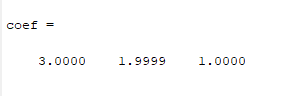
\includegraphics{3b.png}\\
        Thus, we obtain the same results as the Vandermonde matrix. 
    \end{enumerate}
\end{enumerate}

\end{document}